\hypertarget{interacting-quantum-many-body-systems}{%
\section{Interacting Quantum Many Body Systems}\label{interacting-quantum-many-body-systems}}

When you take many objects and let them interact together, it is often simpler to describe the behaviour of the group differently than one would describe the individual objects. Consider a flock (technically called a \emph{murmuration}) of starlings like \cref{fig:Studland_Starlings}. Watching the flock you'll see that it has a distinct outline, that waves of density will sometimes propagate through the closely packed birds and that the flock seems to respond to predators as a distinct object. The natural description of this phenomena is couched in terms of the flock rather than the individual birds.

The behaviours of the flock are an emergent phenomena. The starlings are only interacting with their immediate six or seven neighbours \autocite{king2012murmurations,balleriniInteractionRulingAnimal2008}. This is what a physicist would call a \emph{local interaction}. There is much philosophical debate about how exactly to define emergence \autocite{andersonMoreDifferent1972,kivelsonDefiningEmergencePhysics2016} but for our purposes it enough to say that emergence is the fact that the aggregate behaviour of many interacting objects may be very different from the individual behaviour of those objects.

\hypertarget{fig:Studland_Starlings}{%
\begin{figure}
\centering
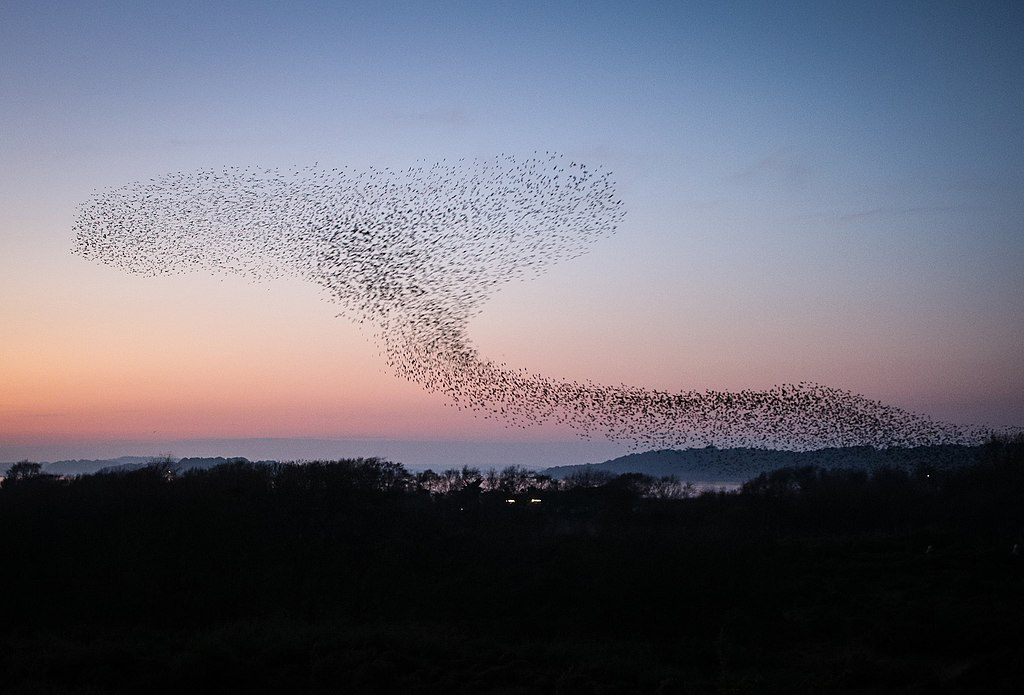
\includegraphics[width=1\textwidth,height=\textheight]{figure_code/intro_chapter/Studland_Starlings.jpeg}
\caption[{A murmuration of Starlings}]{A murmuration of starlings. Dorset, UK. Credit \href{twitter.com/arripay}{Tanya Hart}, ``Studland Starlings'', 2017, \href{creativecommons.org/licenses/by-sa/3.0/deed.en}{CC BY-SA 3.0}}
\label{fig:Studland_Starlings}
\end{figure}
}

To give another example, our understanding of thermodynamics began with bulk properties like heat, energy, pressure and temperature \autocite{saslowHistoryThermodynamicsMissing2020}. It was only later that we gained an understanding of how these properties emerge from microscopic interactions between very large numbers of particles \autocite{flammHistoryOutlookStatistical1998}.

Condensed Matter is, at its heart, the study of what behaviours emerge from large numbers of interacting quantum objects at low energy. When these three properties are present together: a large number of objects, those objects being quantum and there are interaction between the objects, we call it an interacting quantum many body system. From these three ingredients nature builds all manner of weird and wonderful materials.

Historically, we made initial headway in the study of many-body systems, ignoring interactions and quantum properties. The ideal gas law and the Drude classical electron gas \autocite{ashcroftSolidStatePhysics1976} are good examples. Including interactions into many-body physics leads to the Ising model \autocite{isingBeitragZurTheorie1925}, Landau theory \autocite{landau2013fluid} and the classical theory of phase transitions \autocite{jaegerEhrenfestClassificationPhase1998}. In contrast, condensed matter theory got it state in quantum many-body theory. Bloch's theorem \autocite{blochÜberQuantenmechanikElektronen1929} predicted the properties of non-interacting electrons in crystal lattices, leading to band theory. In the same vein, advances were made in understanding the quantum origins of magnetism, including ferromagnetism and antiferromagnetism \autocite{MagnetismCondensedMatter}.

However, at some point we had to start on the interacting quantum many body systems. Some phenomena cannot be understood without a taking into account all three effects. The canonical examples are superconductivity \autocite{MicroscopicTheorySuperconductivity}, the fractional quantum hall effect \autocite{feldmanFractionalChargeFractional2021} and the Mott insulators \autocite{mottBasisElectronTheory1949,fisherMottInsulatorsSpin1999}. We will discuss the latter in more detail.

Electrical conductivity, the bulk movement of electrons, requires both that there are electronic states very close in energy to the ground state and that those states are delocalised so that they can contribute to macroscopic transport. Band insulators are systems whose Fermi level falls within a gap in the density of states and thus fail the first criteria. Anderson Insulators have only localised electronic states near the fermi level and therefore fail the second criteria. We will discuss Anderson insulators and disorder in a later section.

Both band and Anderson insulators occur without electron-electron interactions. Mott insulators, by contrast, are by these interactions and hence elude band theory and single-particle methods.

\hypertarget{fig:venn_diagram}{%
\begin{figure}
\centering
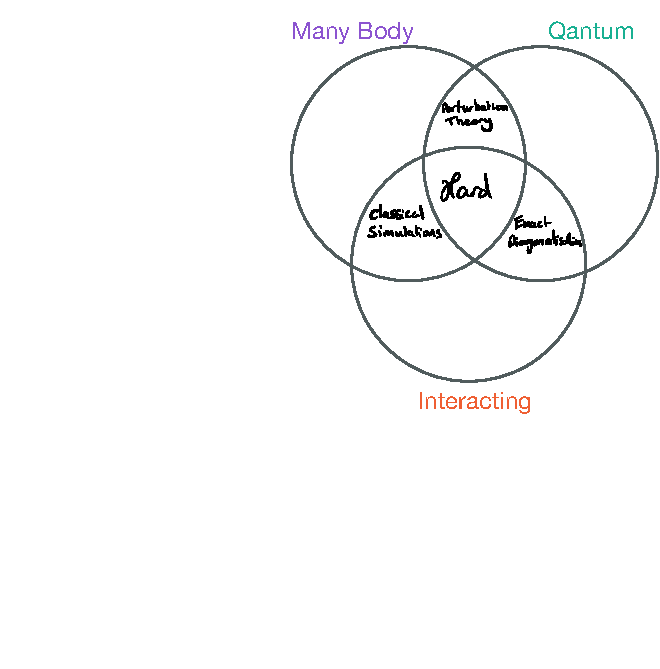
\includegraphics[width=1\textwidth,height=\textheight]{figure_code/intro_chapter/venn_diagram}
\caption[{Interacting Quantum Many Body Systems Venn Diagram}]{Three key adjectives. Many Body, the fact of describing systems in the limit of large numbers of particles. Quantum, objects whose behaviour requires quantum mechanics to describe accurately. Interacting, the constituent particles of the system affect one another via forces, either directly or indirectly. When taken together, these three properties can give rise to what are called strongly correlated materials.}
\label{fig:venn_diagram}
\end{figure}
}

\hypertarget{mott-insulators-and-the-hubbard-model}{%
\section{Mott Insulators and The Hubbard Model}\label{mott-insulators-and-the-hubbard-model}}

The theory of Mott insulators developed out of the observation that many transition metal oxides are erroneously predicted by band theory to be conductive \autocite{boerSemiconductorsPartiallyCompletely1937} leading to the suggestion that electron-electron interactions were the cause of this effect \autocite{mottDiscussionPaperBoer1937}. Interest grew with the discovery of high temperature superconductivity in the cuprates in 1986 \autocite{bednorzPossibleHighTcSuperconductivity1986} which is believed to arise as the result of doping a Mott insulator state \autocite{leeDopingMottInsulator2006}.

The canonical toy model of the Mott insulator is the Hubbard model \autocite{gutzwillerEffectCorrelationFerromagnetism1963,kanamoriElectronCorrelationFerromagnetism1963,hubbardj.ElectronCorrelationsNarrow1963} of \(1/2\) fermions hopping on the lattice with hopping parameter \(t\) and electron-electron repulsion \(U\)

\[ H = -t \sum_{\langle i,j \rangle \alpha} c^\dagger_{i\alpha} c_{j\alpha} + U \sum_i n_{i\uparrow} n_{i\downarrow} - \mu \sum_{i,\alpha} n_{i\alpha}\]

where \(c^\dagger_{i\alpha}\) creates a spin \(\alpha\) electron at site \(i\) and the number operator \(n_{i\alpha}\) measures the number of electrons with spin \(\alpha\) at site \(i\). In the non-interacting limit \(U << t\), the model reduces to free fermions and the many-body ground state is a separable product of Bloch waves filled up to the Fermi level. In the interacting limit \(U >> t\) on the other hand, the system breaks up into a product of local moments, each in one the four states \(|0\rangle, |\uparrow\rangle, |\downarrow\rangle, |\uparrow\downarrow\rangle\) depending on the filing.

The Mott insulating phase occurs at half filling \(\mu = \tfrac{U}{2}\) where there is one electron per lattice site \autocite{hubbardElectronCorrelationsNarrow1964}. Here the model can be rewritten in a symmetric form \[ H = -t \sum_{\langle i,j \rangle \alpha} c^\dagger_{i\alpha} c_{j\alpha} + U \sum_i (n_{i\uparrow} - \tfrac{1}{2})(n_{i\downarrow} - \tfrac{1}{2})\]

The basic reason that the half filled state is insulating seems is trivial. Any excitation must include states of double occupancy that cost energy \(U\), hence the system has a finite bandgap and is an interaction driven Mott insulator. Originally it was proposed that antiferromagnetic order was a necessary condition for the Mott insulator transition \autocite{mottMetalInsulatorTransitions1990} but later examples were found without magnetic order \textbf{cite}.

Various theoretical treatments of the Hubbard model have been made, including those based on Fermi liquid theory, mean field treatments, the local density approximation (LDA) \autocite{slaterMagneticEffectsHartreeFock1951} and dynamical mean-field theory \autocite{greinerQuantumPhaseTransition2002}. None of these approaches is perfect. Strong correlations are poorly described by the Fermi liquid theory and the LDA approaches while mean field approximations do poorly in low dimensional systems. This theoretical difficulty has made the Hubbard model a target for cold atom simulations \autocite{mazurenkoColdatomFermiHubbard2017}.

From here the discussion will branch two directions. First, we will discuss a limit of the Hubbard model called the Falikov Kimball Model. Second, we will go down the rabbit hole of strongly correlated systems without magnetic order. This will lead us to Quantum spin liquids and the Kitaev honeycomb model.

\textbf{An exactly solvable model of the Mott Insulator} - demonstrate mott insulator in hubbard model, briefly tease the falikov kimball model in order to lay the ground work to talk about the falikov kimball model later

\begin{itemize}
\tightlist
\item
  FK model has extensively many conserved charges which makes it tractable
\item
  Disorder free localisation
\end{itemize}

\textbf{An exactly solvable Quantum Spin Liquid} - relationship between mott insulators and spin liquids: the electrons in a mott insulator form local moments that normally form an AFM ground state but if they don't, due to frustration or other reason, the local moments may form a QSL at T=0 instead. \autocite{law1TTaS2QuantumSpin2017,ribakGaplessExcitationsGround2017}

\begin{itemize}
\item
  QSLs introduced by anderson 1973 \autocite{andersonResonatingValenceBonds1973}
\item
  Spin orbit effect is a relativistic effect that couples electron spin to orbital angular moment. Very roughly, an electron sees the electric field of the nucleus as a magnetic field due to its movement and the electron spin couples to this.
\item
  can be string in heavy elements
\item
  The Kitaev Model
\item
  Kitaev model has extensively many conserved charges too
\item
  Frustration
\item
  anyons
\item
  fractionalisation
\item
  Topology -\textgreater{} GS degeneracy depends on the genus of the surface
\item
  the chern number
\item
  quasiparticles
\item
  topological order
\item
  protected edge states
\item
  Abelian and non-Abelian anyons
\end{itemize}

\hypertarget{fig:correlation_spin_orbit_PT}{%
\begin{figure}
\centering
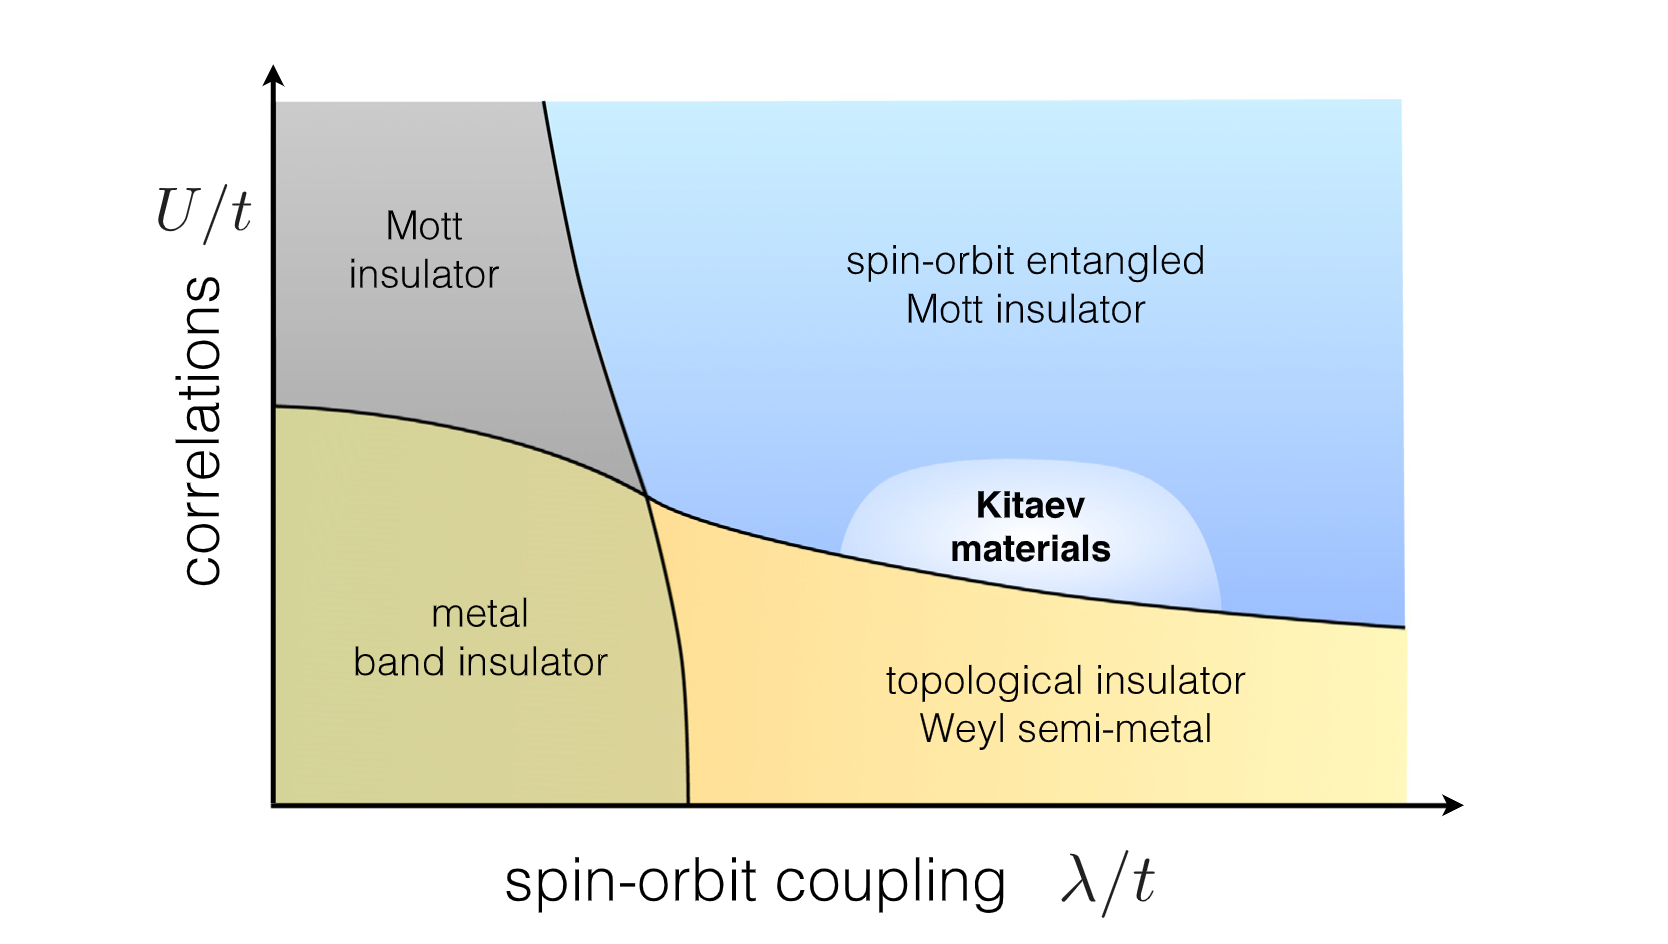
\includegraphics[width=1\textwidth,height=\textheight]{figure_code/intro_chapter/correlation_spin_orbit_PT.png}
\caption[{Phase Diagram}]{From \autocite{TrebstPhysRep2022}.}
\label{fig:correlation_spin_orbit_PT}
\end{figure}
}

kinds of mott insulators: Mott-Heisenberg (AFM order below Néel temperature) Mott-Hubbard (no long-range order of local magnetic moments) Mott-Anderson (disorder + correlations) Wigner Crystal

\hypertarget{outline}{%
\section{Outline}\label{outline}}

This thesis is composed of two main studies of separate but related physical models, The Falikov-Kimball Model and the Kitaev-Honeycomb Model. In this chapter I will discuss the overarching motivations for looking at these two physical models. I will then review the literature and methods that are common to both models.

In Chapter 2 I will look at the Falikov-Kimball model. I will review what it is and why we would want to study it. I'll survey what is already known about it and identify the gap in the research that we aim to fill, namely the model's behaviour in one dimension. I'll then introduce the modified model that we came up with to close this gap. I will present our results on the thermodynamic phase diagram and localisation properties of the model

In Chapter 3 I'll study the Kitaev Honeycomb Model, following the same structure as Chapter 2 I will motivate the study, survey the literature and identify a gap. I'll introduce our Amorphous Kitaev Model designed to fill this gap and present the results.

Finally in chapter 4 I will summarise the results and discuss what implications they have for our understanding interacting many-body quantum systems.
